\subsection{Software Design Considerations}

\todo{remove notes}
(10, 2100 w)

Has the student clearly described the design of their system? Is it described
in sufficient detail to make it easy for someone else to replicate the system?

Has the student justified the design decisions, and discussed alternatives that
were considered?

\todo{Move algorithm to implementation}

\subsubsection{Road Network}
\label{sec:design:network}

A real world road network is represented as a weighted connected graph
constructed of edges (roads) and vertices (origins/destinations). Each vertex
has associated properties: a list of connected edges with their lengths
(weights), a list of passengers, potentially a list of taxis. Each edge has
associated properties: length, potentially speed limit and toll. Taxis can
travel between vertices using edges. Taxis are assumed to take the shortest
routes and travel at a constant speed. Passengers appear at nodes and when taxi
is at a node it is assumed that they can interact, and the passengers wait for
a set amount of time.

Road networks have a specific structure that is different from generic randomly
generated graphs. \textcite{Eisenstat2011graphs+quadtree} believes that the
structure of the graphs is important for optimisation problems, giving the
example of optimising logistics operations for a fleet of vehicles where
algorithmic performance greatly differs from that on generic graphs. Uniform
planar graphs are a reasonably realistic way to represent road networks
\parencite{Eisenstat2011graphs+quadtree, Masucci2009graphs+london}. A way to
generate random planar graphs is suggested by
\textcite{Brinkmann2007graphs+generate}, for which ready-to-use software called
\textit{plantri} is available.

Shortest paths in graphs can be calculated by Djikstra's algorithm
\parencite{Cormen2009algorithms}. However, calculating all possible shortest
paths is not necessary as some routes could never be travelled. Furthermore,
that may be unfeasible in a very large network as the number of paths grows
exponentially. Online calculation of a shortest path between two nodes in a
graph can be efficiently done using \textit{A-star} algorithm by
\textcite{Hart1968paths}.


\subsubsection{Q-Learner}
\label{sec:design:ai}

State is based on the origin, passenger and intended destination. Actions a
taxi can take is enquiring a passenger for destination, offering a price or
driving to another place. If the passenger accepts the price, taxi drives the
passenger to the destination and receives a reward. Keeping track of the exact
passenger is not important. Each time step has a negative reward based on what
action the taxi is taking, always depending on time but also could depend on
distance travelled. The probability of the passenger accepting the fare is the
transition probability. This specifies the research problem as a finite MDP
according to the definition in Section \ref{sec:literature:ai:mdp} (although it
can be argued that prices could theoretically be a continuous space, in reality
they are not).

As described in section \ref{sec:requirements:ai}, Q-Learner is a simple and
adequate reinforcement learning method fit for the project. Of course, the very
basic Q-Learner will need to be extended to accomodate exploration in this
paricular case of having an active agent (see Section
\ref{sec:lit:ai:exploration}. Therefore an exploration constant \(\varepsilon\)
needs to be used for action selection, and it can stay fixed as the horizon for
the simulation will normally be unknown.

A further addition required for the Q-Learner is a step-size function. This
function is used to adjust for the bias of previous estimates. As a state is
being visited more and more, any new experiences are less and less important
compared to the old experiences, therefore the TD weights should be adjusted
less. This issue was discussed in more detail by
\textcite{Sutton1994ai+stepsize}, where three different algorithms are
introduced for optimising the step sizes for improved reinforcement learning
performance. Nevertheless, the policy will still converge even if the step size
simply decays (i.e \(\lim_{n \to \inf}\alpha(n) = 0\) where \(n\) is the number
of times a state has been visited). Therefore for simplicity the function can
be fixed as \(\alpha(n)=\frac{1}{n}\).

When the step size function is added to a basic Q-Learner, the algorithm
adapted from \textcite{Sutton1998ai+reinforcement} can be used as shown in
Algorithm \ref{algorithm:q}. This algorithm updates action-state pair value
estimates, and the learner can then select the optimal action depending on the
exploration function (not shown here).

\begin{algorithm}
  \caption{
  Q-learning. Algorithm that needs to be called after each transition. 
  Adapted from \textcite{Sutton1998ai+reinforcement}. 
  \label{algorithm:q}}

  \begin{algorithmic}[1]
    \Require 
      \Statex $s$ is the last state,
      \Statex $s'$ is the next state,
      \Statex $a$ is the last action,
      \Statex $A(s)$ is a set of actions for a state,
      \Statex $R$ is the immediate reward received,
      \Statex $Q$ is an array hosting the current action-value estimate
      \Statex $H$ is the visit history of state-action pairs,
      \Statex $\alpha$ is a step-size function,
      \Statex $\gamma$ is a discount factor.

      \Statex Policy $Q(s, a)$ is initialised arbitrarily
      \Statex History $H$ is empty

    \Function{Q\_learning}{$s,a,R,a'$}
      \State $\delta \gets R + 
              \gamma \cdot max_{a' \in A(s')} Q(s', a') - Q(s, a)$
      \State $Q(s, a) \gets Q(s, a) + \alpha \cdot \delta$
      \State $H(s, a) \gets H(s, a) + 1$
      \Return $Q, H$      
    \EndFunction
  \end{algorithmic}

\end{algorithm}

\subsection{Architecture} 
\label{sec:design:architecture}

Expressing the simulation design in Section \ref{sec:requirements} and
other software-related considerations discussed in sections
\ref{sec:design:network} and \ref{sec:design:ai}

Global properties: time; Taxis
can enquire for the route from A to B at a small cost, and receive distance.
When taxis decide to go from A to B, they go at a constant speed for the
calculated time. No actions can be taken and they are marked as travelling.

Network of nodes, not known to taxi as a whole

Node has a list of neighbours and distances.
Node has a list of present passengers and taxis.

Taxi model: fixed cost (per unit of time) and variable costs (per unit of
distance), has a set of actions.

Passenger model: probabilistic properties with set relative weights to
calculate demand, responds to bids with Y/N.

Preliminary software class diagram is shown in Figure
\ref{figure:design:software}. \todo{too much detail}

\begin{figure}
  \begin{center}
    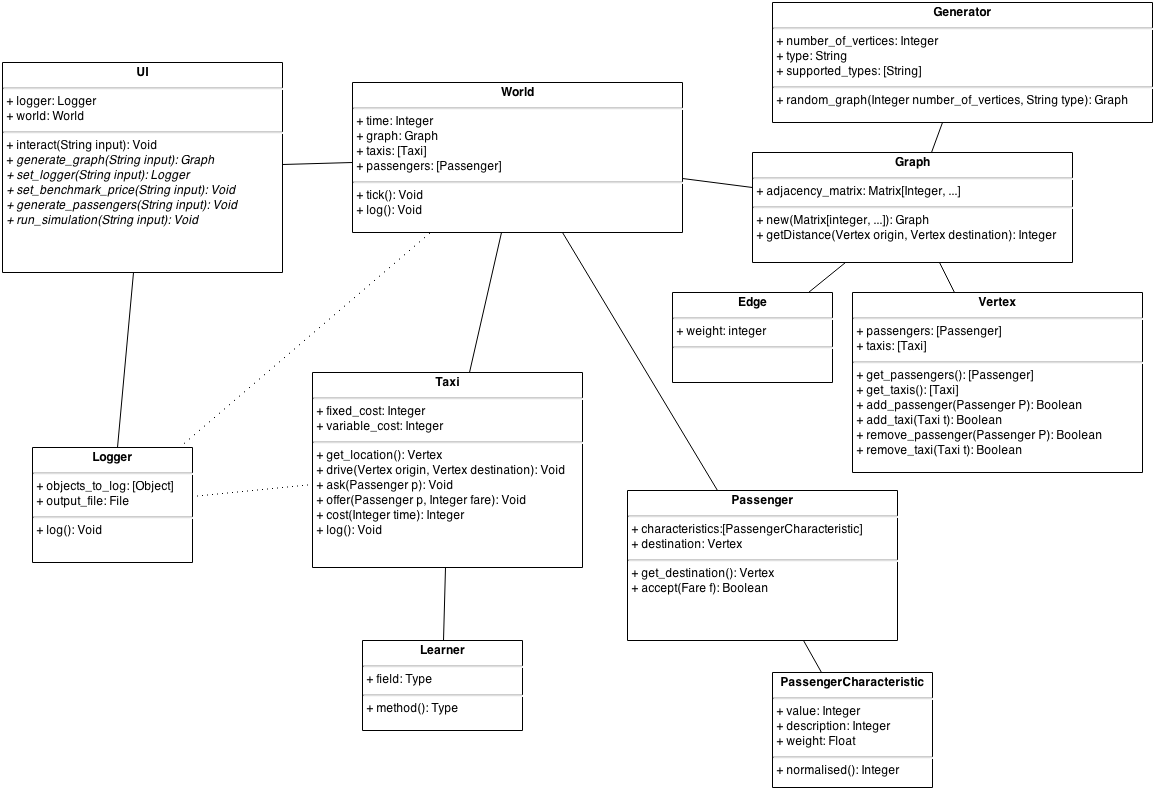
\includegraphics[width=\textwidth]{../figures/software_diagram}
    \caption{
      Software diagram
      \label{figure:design:software}
    }
  \end{center}
\end{figure}
